\chapter{Video}
\renewcommand{\kapitelautor}{Autor: Kerstin Schön}
\section{Interview mit dem Abteilungsvorstand}
\subsection{Idee}
Die Intention des Interviews mit dem Abteilungsvorstand, Dr. Hager, war es, Interessenten allgemeine Informationen über die Schule näher zu bringen. Das Ziel war es, die wichtigsten Informationen kurz und prägnant rüberzubringen, sodass der Interessent die wichtigsten Informationen, ohne lang danach zu suchen, erhält.
\begin{figure}[H]
	\centering	
	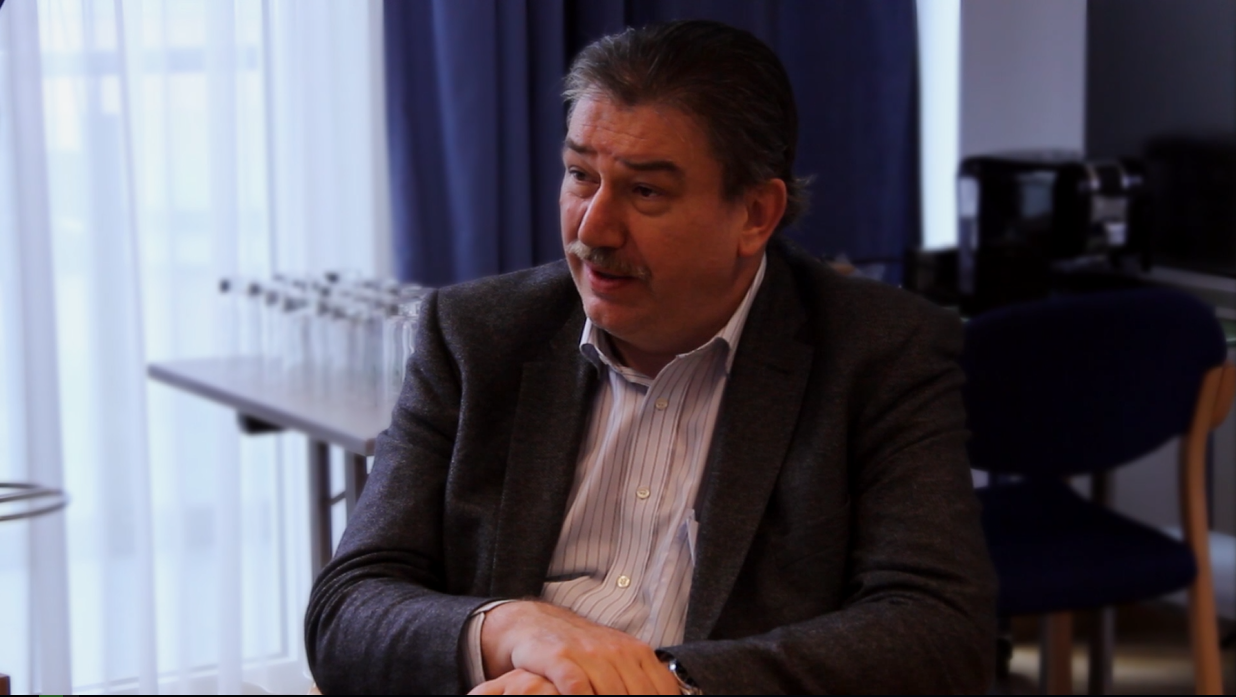
\includegraphics[width=0.8\textwidth]{abb23} 
	\caption{Interview mit dem Abteilungsvorstand}
\end{figure}
\section{Tag der offenen Tür}
\subsection{Idee}
Das Tag der offenen Tür Video dreht sich um die Interessenten, die sich die Schule am Tag der offenen Tür angeschaut haben. Hierbei wurden Fragen, wie: "Wie ist dein erster Eindruck von der Schule?", oder "Kannst du dir vorstellen dich hier anzumelden?" gestellt. Weiters redet am Ende des Videos ein Lehrer über die Schule und erklärt den Unterschied zwischen einer HTL und einer AHS.
\begin{figure}[H]
	\centering	
	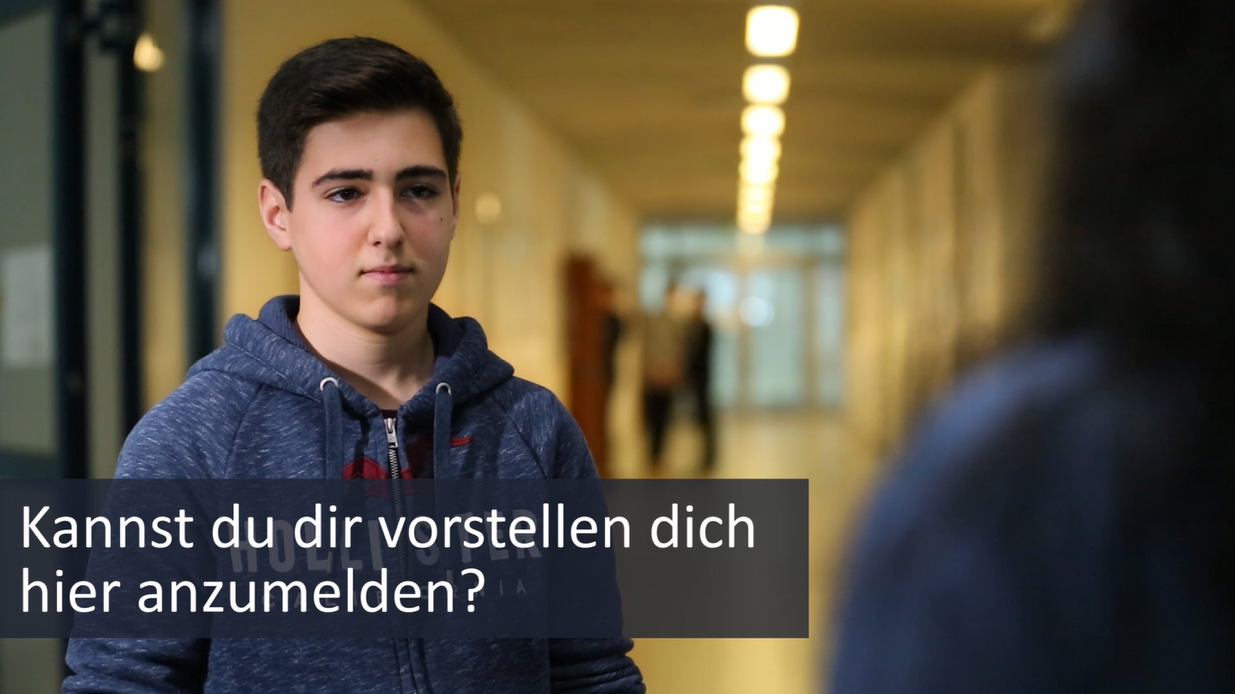
\includegraphics[width=0.8\textwidth]{abb24} 
	\caption{Tag der offenen Tür}
\end{figure}
\section{Video mit einem Absolvent}
\subsection{Idee}
In dem Video, beziehungsweise dem Quiz, mit dem Absolventen und dem Schüler der zweiten Klasse geht es darum, dass dem Absolventen und dem Schüler Fragen gestellt werden, wobei sie 45 Sekunden Zeit haben diese zu beantworten. Derjenige, der die Frage falsch beantwortet, muss ein Jelly-Bean essen, wobei man nicht weiß, ob es ein gutes oder ein schlechtes ist. Die Intention dieses Videos ist es zu zeigen, dass die Medientechnik ein enorm großer Bereich ist, bei dem man nicht alles erlernen kann. So spezialisiert sich jeder Schüler meist auf ein Gebiet, das er dann auch dementsprechend gut kann. Was jedoch zu beachten ist, ist, dass die Schüler dennoch die Grundlagen der anderen Medientechnik Themen lernen und auch können.
\begin{figure}[H]
	\centering	
	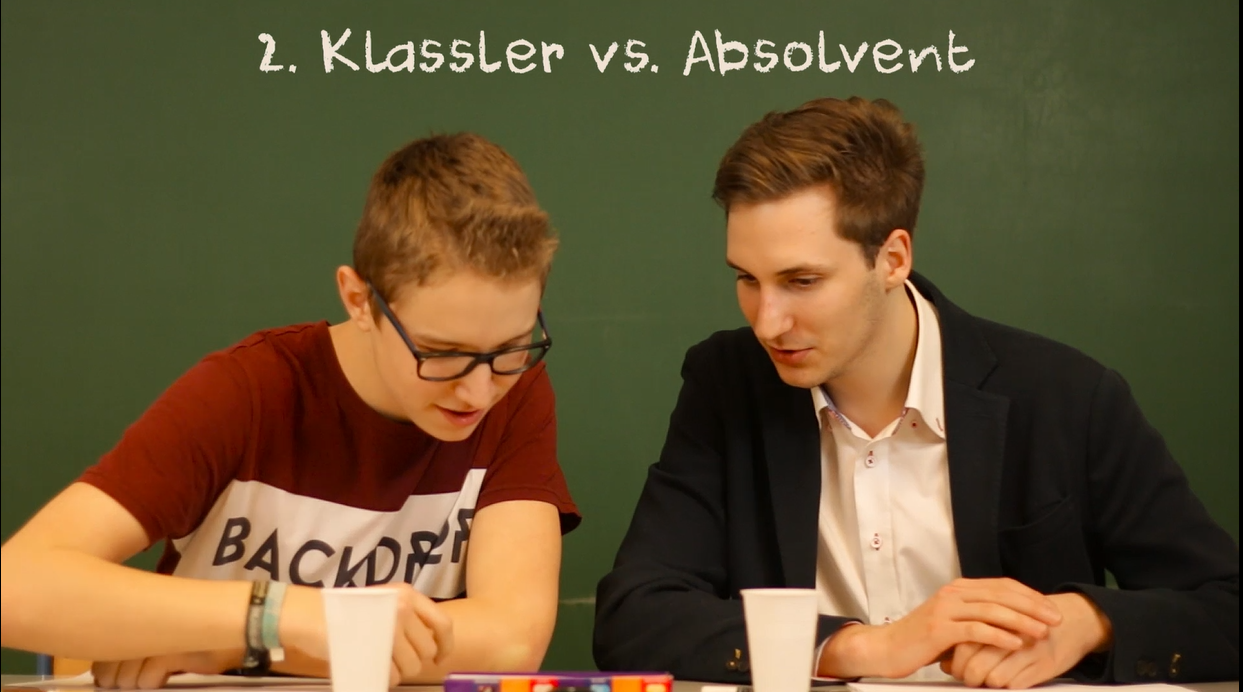
\includegraphics[width=0.8\textwidth]{abb25} 
	\caption{Video mit einem Absolvent}
\end{figure}